\documentclass{article}
\usepackage[paperheight=11in,paperwidth=8.5in,margin=1in]{geometry}
\usepackage{fancyhdr}
\usepackage{graphicx}
\usepackage{float}
\setlength{\headheight}{15.2pt}
\pagestyle{fancy}

\begin{document}
\fancyhf{}
\lhead{Security Crawler}
\chead{MILESTONE 3}
\rhead{\today}

{\large Tasks:}
\begin{enumerate}

\item SSDs 
\begin{figure}[H]
	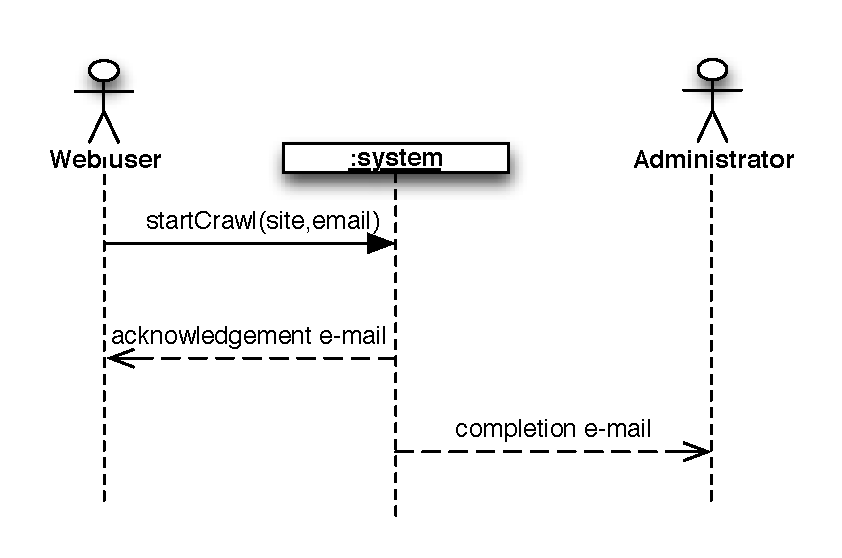
\includegraphics[width=.8\textwidth]{SSD}
	\caption{System Sequence Diagram}
\end{figure}

\newpage

\item OCs\\

{\large \bf Contract 1:} mirrorSite \\[.5cm]
\begin{tabular}{|p{.2\textwidth} | p{.4\textwidth}|}
\hline
Operation: & mirrorSite(address :string, level int) \\ \hline
Cross References: & Use Case: Initiate Web Crawl\\ \hline
Preconditions: &
\begin{itemize}
	\item Site address is known
	\item Site is valid
	\item There is enough space on the hard disk to store the contents of the website
\end{itemize}\\ \hline

Postconditions: &
\begin{itemize}
	\item The website has been mirrored the hard drive
	\item A list of all mirrored files is made
\end{itemize}\\ \hline
\end{tabular} \\[1cm]

{\large \bf Contract 2:} compileVulnList\\[.5cm]
\begin{tabular}{|p{.2\textwidth} | p{.4\textwidth}|}
\hline
Operation: & compileVulnList() \\ \hline
Cross Reference: & Use Case: Display a Trace Log \\ \hline
Preconditions: & 
\begin{itemize}	
	\item All files have been parsed
	\item Certification and server information have been retrieved
	\item There is a file that contains all of the possible vulnerabilities to scan for
\end{itemize} \\ \hline

Postconditions:	&
\begin{itemize}
	\item A list of vulnerabilities is made
	\item The list of vulnerabilities are written to the database
\end{itemize} \\ \hline
\end{tabular}

\newpage
\item Logical Architecture\\
\begin{figure}[H]
	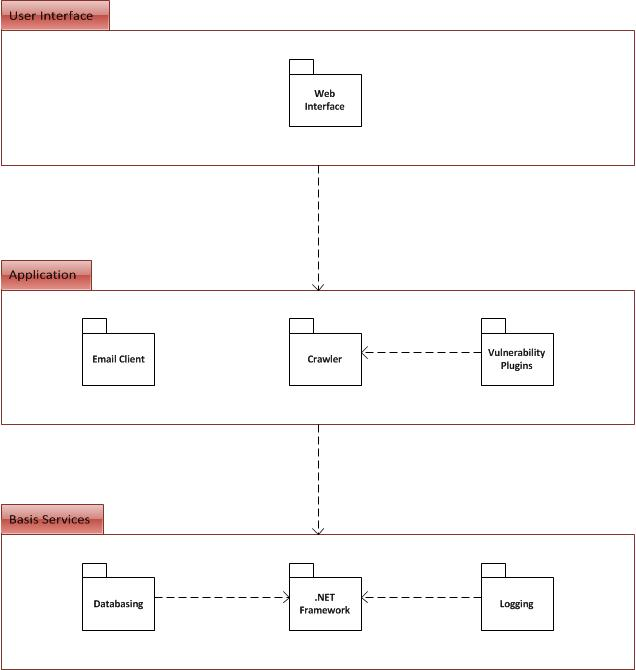
\includegraphics[width=\textwidth]{LogArch}
	\caption{Logical Architecture}
\end{figure}

\newpage
\item Interaction Diagrams\\
\begin{figure}[H]
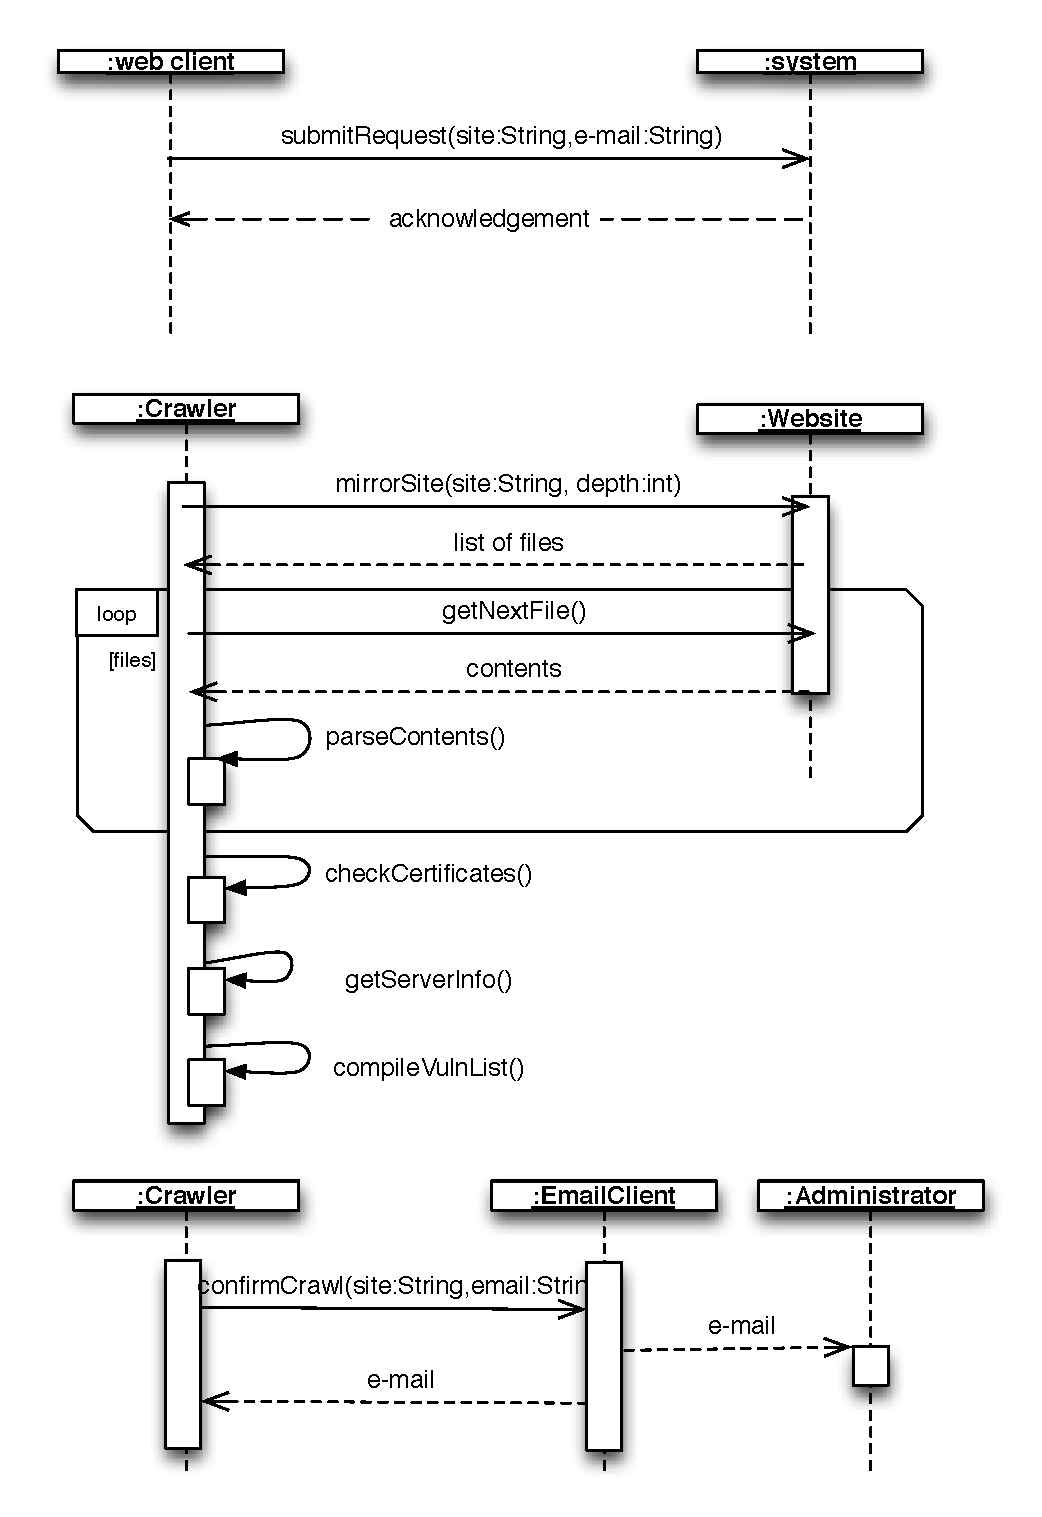
\includegraphics[width=.7\textwidth]{SDs}
\caption{Top to Bottom: SD1: Interaction with web client, SD2:Parsing, SD3: E-mail client and interaction with Administrator}
\end{figure}

\newpage
\item Design Class Diagrams\\
\begin{figure}[H]
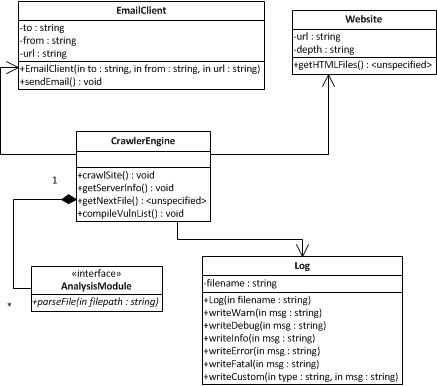
\includegraphics{DCD}
\caption{Design Class Diagram}
\end{figure}

\item Initial Working system\\ (At meeting)
\item Present to customer\\ (To be done 17 Jan)

\end{enumerate}


\end{document}